%
% The MIT License (MIT)
%
% Copyright (c) 2016 Paul Batty
%
% Permission is hereby granted, free of charge, to any person obtaining a copy
% of this software and associated documentation files (the "Software"), to deal
% in the Software without restriction, including without limitation the rights
% to use, copy, modify, merge, publish, distribute, sublicense, and/or sell
% copies of the Software, and to permit persons to whom the Software is
% furnished to do so, subject to the following conditions:
%
% The above copyright notice and this permission notice shall be included in
% all copies or substantial portions of the Software.
%
% THE SOFTWARE IS PROVIDED "AS IS", WITHOUT WARRANTY OF ANY KIND, EXPRESS OR
% IMPLIED, INCLUDING BUT NOT LIMITED TO THE WARRANTIES OF MERCHANTABILITY,
% FITNESS FOR A PARTICULAR PURPOSE AND NONINFRINGEMENT. IN NO EVENT SHALL THE
% AUTHORS OR COPYRIGHT HOLDERS BE LIABLE FOR ANY CLAIM, DAMAGES OR OTHER
% LIABILITY, WHETHER IN AN ACTION OF CONTRACT, TORT OR OTHERWISE, ARISING FROM,
% OUT OF OR IN CONNECTION WITH THE SOFTWARE OR THE USE OR OTHER DEALINGS IN
% THE SOFTWARE.
%

\documentclass[a4paper,12pt]{article}

\usepackage{fancyhdr}						% for headers and footers.
\usepackage{setspace}						% for using single spaces.
\usepackage{mathptmx}						% for Times Roman Closest to Times New Roman.
\usepackage{listings}						% for code sections.
\usepackage{color}							% for colouring the code sections.	
\usepackage{graphicx}						% for images.
\usepackage{longtable}						% for large tables.
\usepackage{float}							% for floting points.
\usepackage{chngcntr}						% for numbering scheme
\usepackage[authoryear]{natbib}			% for refrencing.
\usepackage{titlesec}						% for subsubsub sections

\setcounter{secnumdepth}{4}					% subsubsubsections
\titleformat{\paragraph}
{\normalfont\normalsize\bfseries}{\theparagraph}{1em}{}
\titlespacing*{\paragraph}
{0pt}{3.25ex plus 1ex minus .2ex}{1.5ex plus .2ex}

\bibliographystyle{apalike}					% set refencing style
\bibpunct{(}{)}{;}{a}{,}{,}

\counterwithin{table}{section}				% set section number to caption for tables
\counterwithin{figure}{section}			% set section number to caption for figures

\hyphenpenalty 10000						% remove hyphenation at page width
\exhyphenpenalty 10000

\newlength{\wideitemsep}					% reduce the gap in lists
\setlength{\wideitemsep}{.5\itemsep}
\addtolength{\wideitemsep}{-7pt}
\let\olditem\item
\renewcommand{\item}{\setlength{\itemsep}{\wideitemsep}\olditem}

\makeatletter								% remove Refrence Title buit into biblatex.
\renewenvironment{thebibliography}[1]{
      \list{\@biblabel{\@arabic\c@enumiv}}
           {\settowidth\labelwidth{\@biblabel{#1}}
            \leftmargin\labelwidth
            \advance\leftmargin\labelsep
            \@openbib@code
            \usecounter{enumiv}
            \let\p@enumiv\@empty
            \renewcommand\theenumiv{\@arabic\c@enumiv}}
      \sloppy
      \clubpenalty4000
      \@clubpenalty \clubpenalty
      \widowpenalty4000
      \sfcode`\.\@m}
     {\def\@noitemerr
       {\@latex@warning{Empty `thebibliography' environment}}
      \endlist}
\makeatother

\pagestyle{fancy}							% use the fancy theme.
\fancyhead{}								% clear the headers.
\fancyfoot[CE,CO]{\leftmark}				% Put the Section into the footer.
\fancyfoot[LE,RO]{\thepage}					% put the page number into the footer.
\renewcommand{\headrulewidth}{0pt}			% remove the header rule / line.
\renewcommand{\footrulewidth}{0.4pt}		% place the footer rule / line.

\renewcommand{\arraystretch}{1.3}			% extra padding on tables.

\definecolor{dkgreen}{rgb}{0,0.6,0}		% define colours.
\definecolor{gray}{rgb}{0.5,0.5,0.5}		
\definecolor{mauve}{rgb}{0.58,0,0.82}
\definecolor{backcolour}{rgb}{0.95,0.95,0.92}
\definecolor{numbercolour}{rgb}{0.4,0.4,0.4}

\lstset{frame=tb,							% Set up code section settings.
  language=Java,							% language is java.
  aboveskip=3mm,							% top padding text.
  belowskip=3mm,							% bottom padding between text.
  showstringspaces=true,					% remove space characters.
  columns=flexible,							% flexible columns.
  basicstyle={\small\ttfamily},			% font.
  numbers=left,								% show line numbers on the left.
  numbersep=5pt, 							% size of line numbers.
  frame = false,							% remove the frame.
  backgroundcolor=\color{backcolour}, 		% set the colours.
  numberstyle=\tiny\color{gray},
  keywordstyle=\color{blue},
  commentstyle=\color{dkgreen},
  stringstyle=\color{mauve},
  numberstyle=\color{numbercolour},
  breaklines=false,							% don't break lines.
  breakatwhitespace=false,					% allow whitespace.
  tabsize=4									% set tab size.
}

\input{glyphtounicode}						% enable unicode.
\pdfgentounicode=1
\singlespacing								% enable single spaces.
\setlength{\parindent}{0cm}					% remove indentation.

\begin{document}
	%
% The MIT License (MIT)
%
% Copyright (c) 2017 Paul Batty
%
% Permission is hereby granted, free of charge, to any person obtaining a copy
% of this software and associated documentation files (the "Software"), to deal
% in the Software without restriction, including without limitation the rights
% to use, copy, modify, merge, publish, distribute, sublicense, and/or sell
% copies of the Software, and to permit persons to whom the Software is
% furnished to do so, subject to the following conditions:
%
% The above copyright notice and this permission notice shall be included in
% all copies or substantial portions of the Software.
%
% THE SOFTWARE IS PROVIDED "AS IS", WITHOUT WARRANTY OF ANY KIND, EXPRESS OR
% IMPLIED, INCLUDING BUT NOT LIMITED TO THE WARRANTIES OF MERCHANTABILITY,
% FITNESS FOR A PARTICULAR PURPOSE AND NONINFRINGEMENT. IN NO EVENT SHALL THE
% AUTHORS OR COPYRIGHT HOLDERS BE LIABLE FOR ANY CLAIM, DAMAGES OR OTHER
% LIABILITY, WHETHER IN AN ACTION OF CONTRACT, TORT OR OTHERWISE, ARISING FROM,
% OUT OF OR IN CONNECTION WITH THE SOFTWARE OR THE USE OR OTHER DEALINGS IN
% THE SOFTWARE.
%

\begin{titlepage}
	\begin{center}
		\begin{huge}
			\textbf{Continuous Deployment: A look at Architecture}
		\end{huge}	
		
		
		\vspace{3cm}		
		
		\normalsize By:   \\
		\large Paul Batty
		
		\vspace{2.5cm}
		
		\normalsize Supervisor: \\
		\large Manfred Lau
		
		\vspace{1.5cm}
		
		\large March 2017
		
		\vfill 
		
		\normalsize
		The dissertation is submitted to \\
		Lancaster University \\
		As partial fulfilment of the requirements for the degree of \\
		Integrated Masters of Science in Computer Science \\
	\end{center} 
\end{titlepage}

	%
% The MIT License (MIT)
%
% Copyright (c) 2017 Paul Batty
%
% Permission is hereby granted, free of charge, to any person obtaining a copy
% of this software and associated documentation files (the "Software"), to deal
% in the Software without restriction, including without limitation the rights
% to use, copy, modify, merge, publish, distribute, sublicense, and/or sell
% copies of the Software, and to permit persons to whom the Software is
% furnished to do so, subject to the following conditions:
%
% The above copyright notice and this permission notice shall be included in
% all copies or substantial portions of the Software.
%
% THE SOFTWARE IS PROVIDED "AS IS", WITHOUT WARRANTY OF ANY KIND, EXPRESS OR
% IMPLIED, INCLUDING BUT NOT LIMITED TO THE WARRANTIES OF MERCHANTABILITY,
% FITNESS FOR A PARTICULAR PURPOSE AND NONINFRINGEMENT. IN NO EVENT SHALL THE
% AUTHORS OR COPYRIGHT HOLDERS BE LIABLE FOR ANY CLAIM, DAMAGES OR OTHER
% LIABILITY, WHETHER IN AN ACTION OF CONTRACT, TORT OR OTHERWISE, ARISING FROM,
% OUT OF OR IN CONNECTION WITH THE SOFTWARE OR THE USE OR OTHER DEALINGS IN
% THE SOFTWARE.
%

\vspace*{\fill}

\begin{figure}[H]
	\raggedleft
	
\includegraphics[scale=1]{images/dec_head.jpg}
\end{figure}
\vspace{1cm}

\textbf{Name:} Paul Batty\\\\
\textbf{Student ID:} 33423253\\\\
\textbf{Dissertation Title:} Continuous Deployment: A look at Architecture.\\\\
\textbf{Module:} SCC.421 Fourth Year Project (Computer Science) \\\\

I certify that the material contained in this dissertation is my own work and does not contain unreferenced or unacknowledged material. I also warrant that the above statement applies to the implementation of the project and all associated documentation. Regarding the electronically submitted version of this submitted work, I consent to this being stored electronically and copied for assessment purposes, including the Department’s use of plagiarism detection systems in order to check the integrity of assessed work. I agree to my dissertation being placed in the public domain, with my name explicitly included as the author of the work.
\\\\\\
Date:
\\\\
Signed: 
\\\\\\\\

\begin{figure}[H]
	\raggedright
	
\includegraphics[scale=1]{images/dec_foot.jpg}
\end{figure}

\vspace*{\fill}

%\begin{center}
%To get the code and other documents visit the website at: 
%http://www.lancaster.ac.uk/ug/battyp/autotesting
%\end{center}
	%
% The MIT License (MIT)
%
% Copyright (c) 2017 Paul Batty
%
% Permission is hereby granted, free of charge, to any person obtaining a copy
% of this software and associated documentation files (the "Software"), to deal
% in the Software without restriction, including without limitation the rights
% to use, copy, modify, merge, publish, distribute, sublicense, and/or sell
% copies of the Software, and to permit persons to whom the Software is
% furnished to do so, subject to the following conditions:
%
% The above copyright notice and this permission notice shall be included in
% all copies or substantial portions of the Software.
%
% THE SOFTWARE IS PROVIDED "AS IS", WITHOUT WARRANTY OF ANY KIND, EXPRESS OR
% IMPLIED, INCLUDING BUT NOT LIMITED TO THE WARRANTIES OF MERCHANTABILITY,
% FITNESS FOR A PARTICULAR PURPOSE AND NONINFRINGEMENT. IN NO EVENT SHALL THE
% AUTHORS OR COPYRIGHT HOLDERS BE LIABLE FOR ANY CLAIM, DAMAGES OR OTHER
% LIABILITY, WHETHER IN AN ACTION OF CONTRACT, TORT OR OTHERWISE, ARISING FROM,
% OUT OF OR IN CONNECTION WITH THE SOFTWARE OR THE USE OR OTHER DEALINGS IN
% THE SOFTWARE.
%

\section*{\centering Abstract}

This paper looks into continuous deployment with a focus on the architecture of such a system from the ground up. Starting with where it came from, what it is and the technologies used. Then looking at what an ideal continuous deployment system would be all the way from developer to user. With a quick look at the cost-benefits and who would benefit from such a system. Then taking a look at what is missing, seeing that in general the tools and technology used is on the right track and destined for success. However, the embedded systems and continuous deployment seem to be out of sync therefore more tools need to be created to aid this area into being brought up to date with rest.

\vspace{1.5cm}

\textbf{Keywords:} Continuous deployment, Continuous integration, Automated builds, agile, VCS, workflow, Extreme programming 
	%
% The MIT License (MIT)
%
% Copyright (c) 2017 Paul Batty
%
% Permission is hereby granted, free of charge, to any person obtaining a copy
% of this software and associated documentation files (the "Software"), to deal
% in the Software without restriction, including without limitation the rights
% to use, copy, modify, merge, publish, distribute, sublicense, and/or sell
% copies of the Software, and to permit persons to whom the Software is
% furnished to do so, subject to the following conditions:
%
% The above copyright notice and this permission notice shall be included in
% all copies or substantial portions of the Software.
%
% THE SOFTWARE IS PROVIDED "AS IS", WITHOUT WARRANTY OF ANY KIND, EXPRESS OR
% IMPLIED, INCLUDING BUT NOT LIMITED TO THE WARRANTIES OF MERCHANTABILITY,
% FITNESS FOR A PARTICULAR PURPOSE AND NONINFRINGEMENT. IN NO EVENT SHALL THE
% AUTHORS OR COPYRIGHT HOLDERS BE LIABLE FOR ANY CLAIM, DAMAGES OR OTHER
% LIABILITY, WHETHER IN AN ACTION OF CONTRACT, TORT OR OTHERWISE, ARISING FROM,
% OUT OF OR IN CONNECTION WITH THE SOFTWARE OR THE USE OR OTHER DEALINGS IN
% THE SOFTWARE.
%

\section*{Introduction}
\label{sec:introduction}

Continuous deployment in no new idea as the field of computer science strives to automated all that it can. However, the idea and implementation of automating the development pipeline, going under the name of continuous integration and continuous deployment is a ever changing field. This has lead to the rise of devops also known as development operations dedicated to maintaining and building such systems with more of a focus on the collaboration of the different team involved in the pipeline such as quality assurance, development and management.
\\\\
During a recent project tasked with the aim to create the pipeline from the ground up there were many question that had to be answered. Such as what is the difference between continuous integration and continuous deployment. How does each part of the system fit into the big picture. What is the end game of the system. This is covered in the first section of this paper.
\\\\
Besides just understanding the reasoning and terms used behind the names, it was time to design and implement a system for the project. In addition to looking at the project that this idea spawned from, the paper will look at other attempts and experience from both industry and academic to understand the ideal architecture. This is covered in the second and third chapters.
\\\\
From here the paper will look at the how this architecture will work in practise, the patterns and the direction that this field is heading towards making sure that it is on the right track. This is covered in the final sections four and five.
\\\\
During the creation of the project there seemed to be no coherent or common meanings behind some of the terms. There also was a lack of architectural designs and implementations with most arguing about the systems cost-benefits.
\\\\
Therefore, the main aim of this paper is help define and understand the systems and terms used in this field. In addition to looking at the common themes used in practise to provide a guide for the creation of other automated systems, and those looking to understand this area more in depth.

	%
% The MIT License (MIT)
%
% Copyright (c) 2016 Paul Batty
%
% Permission is hereby granted, free of charge, to any person obtaining a copy
% of this software and associated documentation files (the "Software"), to deal
% in the Software without restriction, including without limitation the rights
% to use, copy, modify, merge, publish, distribute, sublicense, and/or sell
% copies of the Software, and to permit persons to whom the Software is
% furnished to do so, subject to the following conditions:
%
% The above copyright notice and this permission notice shall be included in
% all copies or substantial portions of the Software.
%
% THE SOFTWARE IS PROVIDED "AS IS", WITHOUT WARRANTY OF ANY KIND, EXPRESS OR
% IMPLIED, INCLUDING BUT NOT LIMITED TO THE WARRANTIES OF MERCHANTABILITY,
% FITNESS FOR A PARTICULAR PURPOSE AND NONINFRINGEMENT. IN NO EVENT SHALL THE
% AUTHORS OR COPYRIGHT HOLDERS BE LIABLE FOR ANY CLAIM, DAMAGES OR OTHER
% LIABILITY, WHETHER IN AN ACTION OF CONTRACT, TORT OR OTHERWISE, ARISING FROM,
% OUT OF OR IN CONNECTION WITH THE SOFTWARE OR THE USE OR OTHER DEALINGS IN
% THE SOFTWARE.
%

\section{Background}

The following chapter will cover two sections. Firstly, looking at where the idea for continuous development came from and the how the field ended up where it is today, going over the terms used. The second part looking at some of the tools used.

\subsection{History of Continuous deployment}

Continuous deployment is in a group of methodologies under the name of extreme programming (XP) which in turn is part of the Agile process \cite{XP}. The core principles of extreme programming is to be adaptive to change and quick feedback for everyone involved. Developers get feedback on the code, bugs and features. Clients get the features they need and Managers can make decisions about the direction of the project without bringing the whole system down. TODO:cite
\\\\
This movement started in March 1996 by Ken Back TODO:cite with continuous integration going further back to 1991 by Grady Booch TODO:cite. The main change between that of Booch's design and extreme programming, is that Booch placed a one integration a day limit, whereas extreme programming favours much more. TODO:cite
\\\\
The core idea behind Booch's idea is to avoid problems when a new release is integrated into an old system. It could achieve this goal via automated unit tests. Each test would run through a single public method and make sure that it is performing as it should. For example if a method takes two numbers and return the sum of the numbers. A unit test would test that \textit{1+1} will return \textit{2}, trying edge cases such as using letters and so on. In total there would be a group of tests for every public function. 
\\\\
After the developer has made a change to the code base they would run the tests if they all passed then the code was OK to be check in and used in the next release. This was enhanced with the idea of test driven development, where the test are written first then the change.
\\\\
This all started to kick off around 1997 with the continuous integration being place inside of the extreme programming movement.  This continued until 1999 through various books and publications by the movement, namely Kent Beck.
\\\\
Up to this point continuous integration just consisted of developers writing unit tests and running them locally to make sure that everything passes. When all the test pass the developer would then   check in the changes in to the version control system (VCS). Other developer then working on the same code base will be able to get the latest code and know that it works.
\\\\
This started to change around 2001 with the release of CruiseControl, because in the previous system what if a developer did not run the unit tests, or forgot or check in some files, so it would work fine on their local set-up but nowhere else. Therefore rather then leaving it up to the developer it could be automated. This introduced the idea of build servers. 
\\\\
A build server would sit there and depending on the particular set up and work-flow of the project,  would take the changes run the tests against them and then send out a report to the developer, or anyone who was interested. Now the if the developer forgot something it would be caught before anyone else started working on top of the changes.
\\\\
So far most of the work was performed by developers for developers, in order to assure that the current state of the code base was in a always working condition. This continues until 2008 when Patrick Debois and Andrew Shafer meet up and discuss bridging the gap between development, system administrators and other roles within the agile infrastructure. For example the developer environment is different to the test environment witch in turn is different to QA and production environments. 
\\\\
This then sparked the next stage in the movement, the creation of devops. This in turn created a whole host of new tools such as Jenkins (Hudson), Puppet and Chef just to name a few. These new tools made continuous integration easier then ever, and as they gained maturity started to see a lot of use in industry.
\\\\
As these tools started to gain popularity and with the internet being widespread, there was a shift to not only able to test, but as as the code is in a always working condition push out to the customers so they can always have the latest version, features and so on. This goes under the name of continuous deployment. This allows bugs to be fixed almost as quickly as they are found due to the reproduction of the customers environment back over in the developers workstation.
\\\\
Today, the transition over to continuous deployment is still being made, with more tools arriving. The idea of serverless severs and tools such as Docker in order to increase the reproducibility of the environments faster and with better accuracy.
\\\\
In short the entire pipeline is beneficial to everyone and comes in three different levels, automated builds, continuous integration and continuous deployment. Each being a step up from the one before it. 

\subsection{Tools}

In the previous part this paper named various tools that are used in the pipeline, they fall into three large categories, version control systems, testing  and infrastructure. In this next part the paper will look at each of the categories in turn to understand where they fit into the big picture and how they are used.

\subsubsection{Version control systems}

A version control system (VCS) or version control goes under two other names, revision control and source control. A VCS has a simple premise to manage the changes performed on a document. For example every time a document is edited, the changes are stored alongside the timestamp, user and other metadata. Then if at some point down the line a user want to see who made the changes or undo the changes as it broke the system they should be able to easily. 
\\\\
In short it is a system to manage a documents version, over long periods of time even when the system in closed, restarted or moved. This lays the foundations for more complex operations. As the changes are stored comparisons of different versions can be made, allowing them to be merged together.
\\\\
If user A sees an error in a document that the owner has not fixed, they can show the changes to the owner, if the owner agrees and likes the changes they can merge them in. This applies the changes from user A into the main document. This is also known as a pull request.
\\\\
If the owner makes a change to the document they do not need to send a pull request as they own the original, therefore they can merge right away. This merging is also called checking in, as the person is checking in there changes to the VCS.
\\\\
The VCS however, does not just record changes to just a single document but everything inside of a folder. Therefore it will track adding new files, deleting files and renaming files. Each VCS handles it slightly differently, however this is irrelevant to this paper.The folder will the in case of software development be the project root.
\\\\
If a VCS is tracking all files, then when checking in changes it would be a waste to do this per file, instead changes are grouped together under a commit. This commit is then checked in one go. Rather than a single file at a time, this allows relevant changes to be grouped together creating a nicer history for the project.
\\\\
VCS has one more main function to cover in respects to this paper, called branching. Similar to that in a tree VCS have a main or master branch called the trunk. A branch is similar to a workspace, and represents the changes on that workspace that got it to its current point.
\\\\
When branching it creates a copy of the current branch allowing it to take off in a different direction. Therefore development can go into two different directions without issues of people working on the same file. Then if needed can be merged back. This is better represented graphically as seen below in figure \ref{fig:vcs_branching}:

\begin{figure}[H]
	\centering
	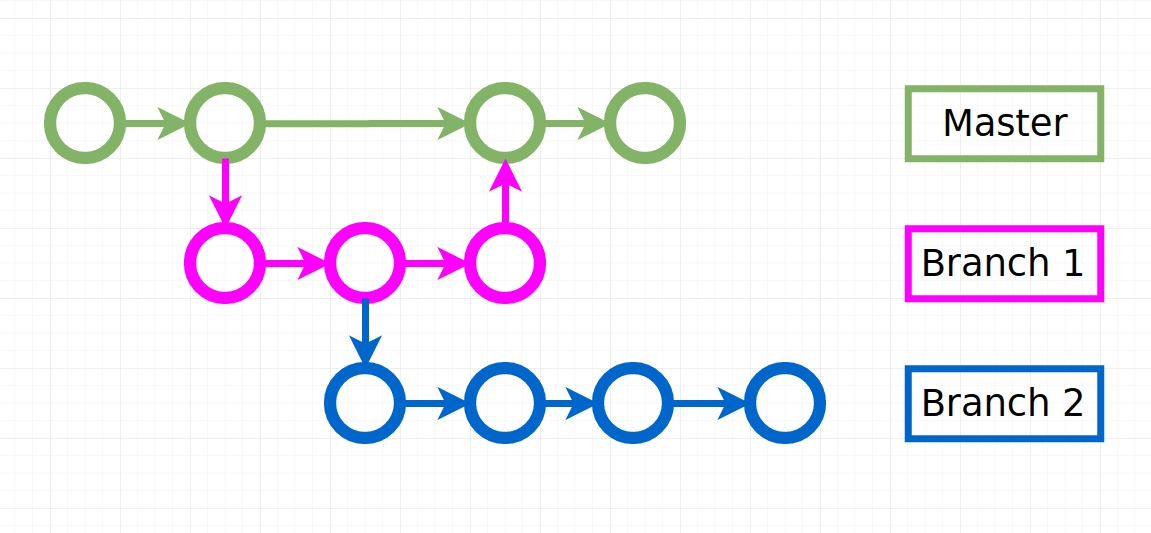
\includegraphics[scale=0.30]{images/branching.jpg}
	\caption{VCS Branching}
	\label{fig:vcs_branching}
\end{figure}

Each circle on the figure represents a commit (a group of changes). The figure also shows that branch one splits off from master, using it as its base then merged back in. While branch two uses branch one as its base, however has not yet been merged. There are different work-flows around this feature covered in more depth in section TODO:link the section.
\\\\
So far the paper has gone on about a folder that exists, this folder goes under the name of a repository. The next part will look at where the repository is located, such that multiple people or a single person can work on the project taking advantage of VCS, and how they differ. There are two main way that this is achieved, both use a client sever architecture. 
\\\\
The first has the server contain the repository, then the developer will create a local copy of the repository according to the branch they are on. They then work on the local copy editing files, however anything else such as creating a branch, merging or checking out files is performed by the server therefore a connection is required.
\\\\
The second way is distributed and has the developer create a local repository that mimic the server one then everything can be performed locally. When a connection to the server is available they can push their changes on the the server repository. This can be seen figure \ref{fig:vcs_systems}:

\begin{figure}[H]
	\centering
	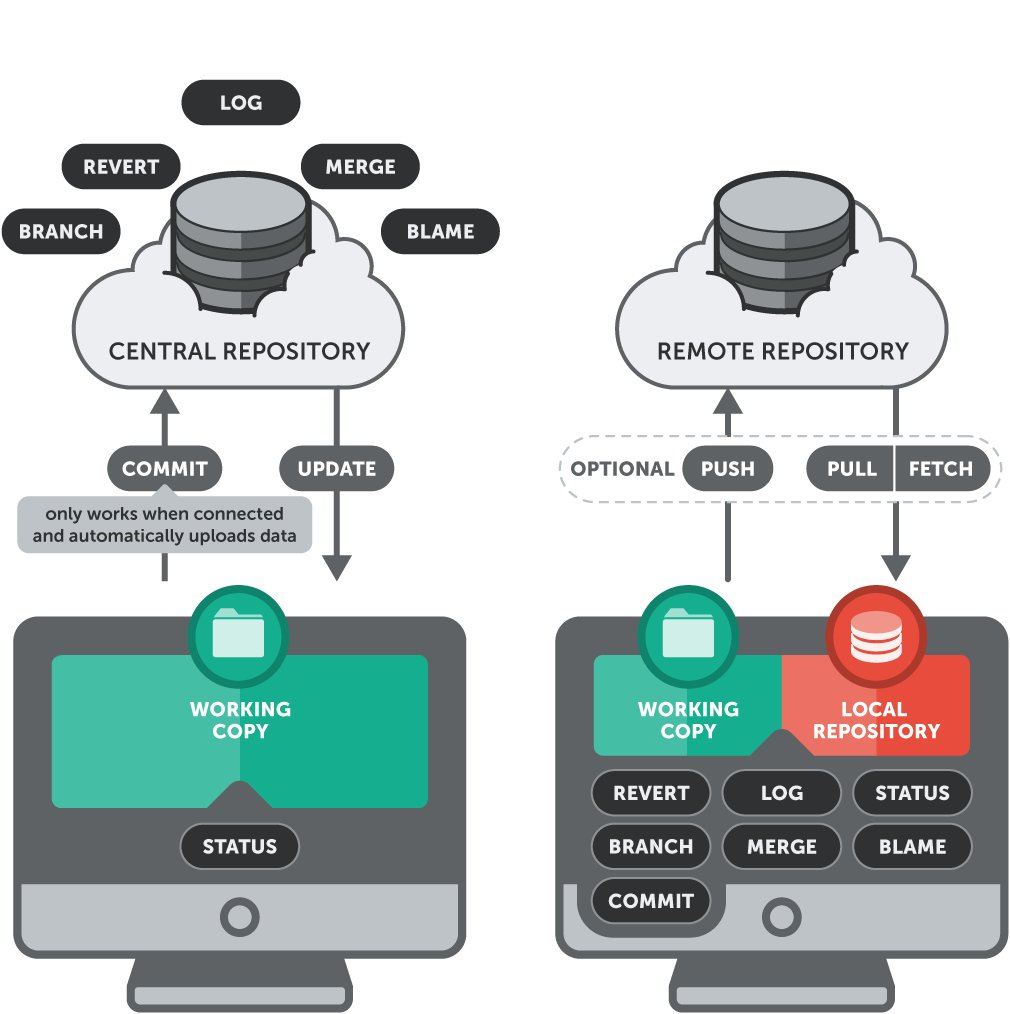
\includegraphics[scale=0.30]{images/systems.jpg}
	\caption{VCS systems modified from \cite{VCSSYSTEMS}}
	\label{fig:vcs_systems}
\end{figure}

There are a lot VCS out there, however the most popular is GIT, TFS and Subversion (\cite{vcspop}). Git follows the distributed system whereas TFS and Subversion uses the repository server system.
\\\\
There are a lot more intricate details to VCS however they will not be covered this paper.

\subsubsection{Testing}



\subsubsection{Infrastructure}
	%
% The MIT License (MIT)
%
% Copyright (c) 2017 Paul Batty
%
% Permission is hereby granted, free of charge, to any person obtaining a copy
% of this software and associated documentation files (the "Software"), to deal
% in the Software without restriction, including without limitation the rights
% to use, copy, modify, merge, publish, distribute, sublicense, and/or sell
% copies of the Software, and to permit persons to whom the Software is
% furnished to do so, subject to the following conditions:
%
% The above copyright notice and this permission notice shall be included in
% all copies or substantial portions of the Software.
%
% THE SOFTWARE IS PROVIDED "AS IS", WITHOUT WARRANTY OF ANY KIND, EXPRESS OR
% IMPLIED, INCLUDING BUT NOT LIMITED TO THE WARRANTIES OF MERCHANTABILITY,
% FITNESS FOR A PARTICULAR PURPOSE AND NONINFRINGEMENT. IN NO EVENT SHALL THE
% AUTHORS OR COPYRIGHT HOLDERS BE LIABLE FOR ANY CLAIM, DAMAGES OR OTHER
% LIABILITY, WHETHER IN AN ACTION OF CONTRACT, TORT OR OTHERWISE, ARISING FROM,
% OUT OF OR IN CONNECTION WITH THE SOFTWARE OR THE USE OR OTHER DEALINGS IN
% THE SOFTWARE.
%

\section{Study requirements}

From the now understood concepts and ideas presented, the paper will now shift onto the collection of data and compacting them into the final results. 
\\\\
Before stating what data is used and how it is collected some limitation will be placed on the project. Firstly, the data will be limited to that of continuous deployment and continuous integration. With regards to continuous integration, the data will be looked at as a continuous deployment point of view, as for the most part the difference is minuscule.
\\\\
Secondly while the tools used are important the main focus will be on the architecture of the system rather than what they are using, as this is the main focus of the paper.

\subsection{Goals}

Before any data collection could take place several question where outlined to form the foundations of this paper and to define a clear goal to head towards, they as as follows:

\begin{itemize}
  \item Is there a clear or ideal architecture that when creating a new or adapting another system should use or head towards.\\
    \item Where are the common traps and pitfalls found when creating a such a system, interlinked  with goal one what can be changed to avoid them.\\
  \item Does the benefits or creating such a system, in both hours and effort pay of in the end. \\
\end{itemize}

\subsection{Data Collection}

The data collection process can be split into three distinct parts, the first one containing blogs and articles written by others who have implemented, used or worked with continuous deployment systems. This type of information will make up the majority of the data collected as it is intend to collect real world experience of such systems in order to find the flaws and how they were corrected.
\\\\
The second type of of data will be in the form of other research carried out, due to the abjectly questionable nature about the architecture of a perfect system, the majority of papers are based around quantifying the cost-benefits of the systems or how they work in certain areas rather then how they are put together. Therefore it will be a smaller percentage of the collected data.
\\\\
The third type of data will be white papers and papers written by companies, and as such will have a bias to them, however, they will be used in conjunction with the rest in order to offset said bias as much as possible.
\\\\
The rest of the paper from here onwards will be the results gathered from the data collected in order to answer the question above. The following first section will be aimed at the first two goals, with the second part focusing on the final question.
	%
% The MIT License (MIT)
%
% Copyright (c) 2017 Paul Batty
%
% Permission is hereby granted, free of charge, to any person obtaining a copy
% of this software and associated documentation files (the "Software"), to deal
% in the Software without restriction, including without limitation the rights
% to use, copy, modify, merge, publish, distribute, sublicense, and/or sell
% copies of the Software, and to permit persons to whom the Software is
% furnished to do so, subject to the following conditions:
%
% The above copyright notice and this permission notice shall be included in
% all copies or substantial portions of the Software.
%
% THE SOFTWARE IS PROVIDED "AS IS", WITHOUT WARRANTY OF ANY KIND, EXPRESS OR
% IMPLIED, INCLUDING BUT NOT LIMITED TO THE WARRANTIES OF MERCHANTABILITY,
% FITNESS FOR A PARTICULAR PURPOSE AND NONINFRINGEMENT. IN NO EVENT SHALL THE
% AUTHORS OR COPYRIGHT HOLDERS BE LIABLE FOR ANY CLAIM, DAMAGES OR OTHER
% LIABILITY, WHETHER IN AN ACTION OF CONTRACT, TORT OR OTHERWISE, ARISING FROM,
% OUT OF OR IN CONNECTION WITH THE SOFTWARE OR THE USE OR OTHER DEALINGS IN
% THE SOFTWARE.
%

\section{Architecture}

Now that the paper has covered all the concepts and ideas needed to build a full continuous deployment pipeline, this next section aims to look at the different form found in use and how they are put together.

\subsection{Starting point}

So far the paper has mentioned about a pipeline, the pipeline being taking the developers changes and getting then out to the customer in a working order. From a purely simplistic point of view the pipeline will look like the that seen in figure \ref{fig:pipeline-simple}.

\begin{figure}[H]
	\centering
	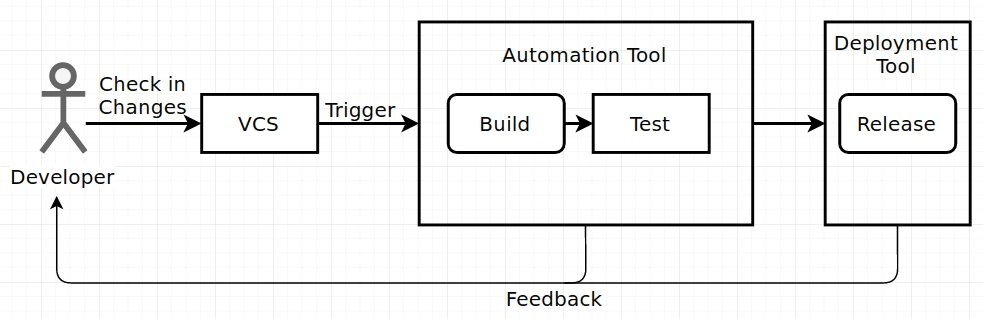
\includegraphics[scale=0.45]{images/pipeline-simple.jpg}
	\caption{The pipeline made simple}
	\label{fig:pipeline-simple}
\end{figure}

The developer will check in the code to the VCS witch in turn will trigger the automation tool. The automation tool will then build the project and test, before sending it out to release. If any of the stages fail the rest of the pipeline is not ran and feedback is sent to the developer so they can fix it.
\\\\
The testing part of the pipeline refers to unit tests and the other forms mentioned in the earlier chapters. Even on a full pass the feedback will be sent, this will help guard against false positives.
\\\\
When talking about the architecture such a system there are two side, firstly the software pipeline as seen above. How each of the steps flow into each over and what is needed to pass between each of the steps. The second is the hardware layout,  such as are the unit tests ran of the same server that it is built, or maybe the entire pipeline in confined to a single server.

\subsection{Software architecture}
\label{sec:testing}

Figure \ref{fig:pipeline-simple} showed a basic pipeline for a continuous delivery pipeline, however there is not enough details to build a system from this. Below figure \ref{fig:bsipipeline} shows the system developed from the project that sparked this paper:

\begin{figure}[H]
	\centering
	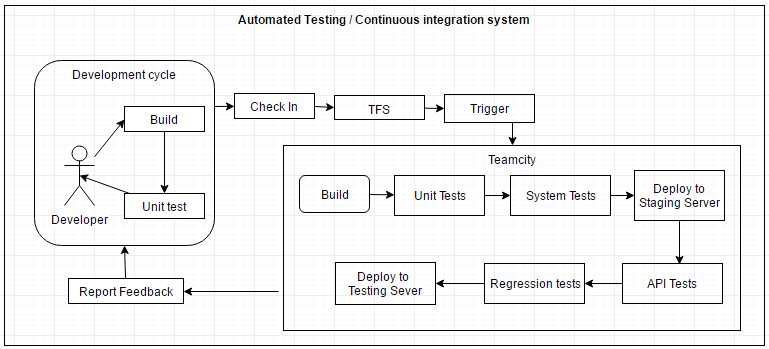
\includegraphics[scale=0.6]{images/bsipipleine.png}
	\caption{A full delivery pipeline}
	\label{fig:bsipipeline}
\end{figure}

The figure shows two things, firstly it reveals the local development cycle. The cycle being that the developer will check the basics before checking in the code to the VCS in this case a TFS server. Not noted on the diagram the developer will also have access to a local running copy of the program allowing them to run other forms of tests if needed. 
\\\\
The second part, it expands on the build and test block previously seen, firstly, the build, then the unit tests followed by system tests. System not mention before are tests a form of integration tests. This then leads on to a interesting part where the system is deployed on a staging instance, this allows the API and regression tests to be ran, as they require a the full system up and running. This is then deployed to testing  for manual tests, where it can then be pushed to production.
\\\\
The interesting part here is how four different deployments are needed, one for the developer, one for staging, one for testing and one for production. This is where Docker and other such tools fit into the picture.
\\\\
This kind of pipeline is a common one, some may use different types of tests as it will suite their needs better, but the theme is still the same. One such system by \cite{zend} adds an additional step after build to package the system up, ready to deploy, and as mentioned they have swapped out the test types for that which suit their product.
\\\\
Another interesting take on this by \cite{codeahoy}, has split their project into different components, this means rather than having one project to handle integration tests, both system to to be build and then integrated together. Therefore they used the architecture in figure \ref{fig:codeahoy}:

\begin{figure}[H]
	\centering
	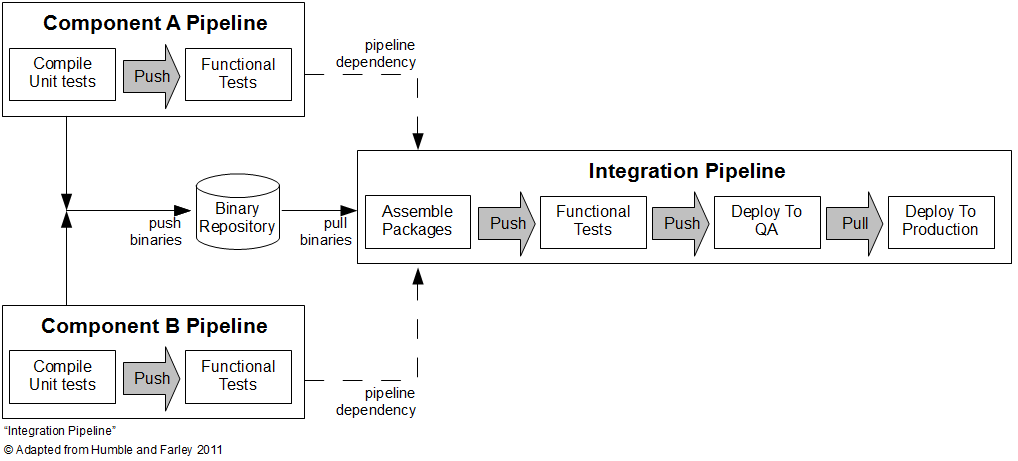
\includegraphics[scale=0.5]{images/codeahoy.png}
	\caption{A dual channel delivery pipeline by \cite{codeahoy}}
	\label{fig:codeahoy}
\end{figure}

This design has added an additional repository for binaries, then when a commit is placed in component A or B, it can progress through the entire pipeline by getting the latest version of the other components binaries from the repository. 
\\\\
\cite{thoughworks} takes this a step further by not only splitting the pipeline into separate components  but also places them in different repositories, making the first time they are integrated together being the integration tests as they all come from their own binary repositories.
\\\\
This kind of pattern goes along with the development environments based on breaking up a monolith architecture of a project into smaller more manageable units. This system makes it easy to add continuous deployment into micro service an other types of modular architecture.
\\\\
One thing not show so far but some teams find invaluable is to run a static analysis on the code base to pre-emptively spot erroneous areas in the project before they happen. This can then be sent back with the rest of the report to the developers and other interested parties.
\\\\
This basic pattern and flow of the pipeline does seems to be a common theme throughout all over implementations.  With the single monolith structure taking it from the start to end and the second combining multiple components into a single software package. 

\subsection{VCS workflow}
\label{sec:vcs}

As seen the pipeline is generally triggered via a commit into the VCS this makes the workflow with the branch structure and VCS a central component into how the rest of the systems are put together.
\\\\
There are two main schools of thoughts when working with continuous deployment and VCS the first is more commonly seen in open source projects that are hosted on sites such as Github and Bitbucket, with the second when everyone has full access to the repository. 
\\\\
The fist uses a pull request system, all the developers or contributes to the project will submit their changes trough a pull request. When the request is made an automated system will start the process of running through the pipeline. 
\\\\
Here the system can automatically merge the change if it passes, however, in open source project it is more common to find the owners to perform a code review and check for harmful changes before merging the request manually. If however it is a private repository the code checked in can be automatically merged. 
\\\\
If the checks fail the request can remain open util an update is pushed to it where it will run the checks again. This is visualised in figure \ref{fig:osspipeline}.

\begin{figure}[H]
	\centering
	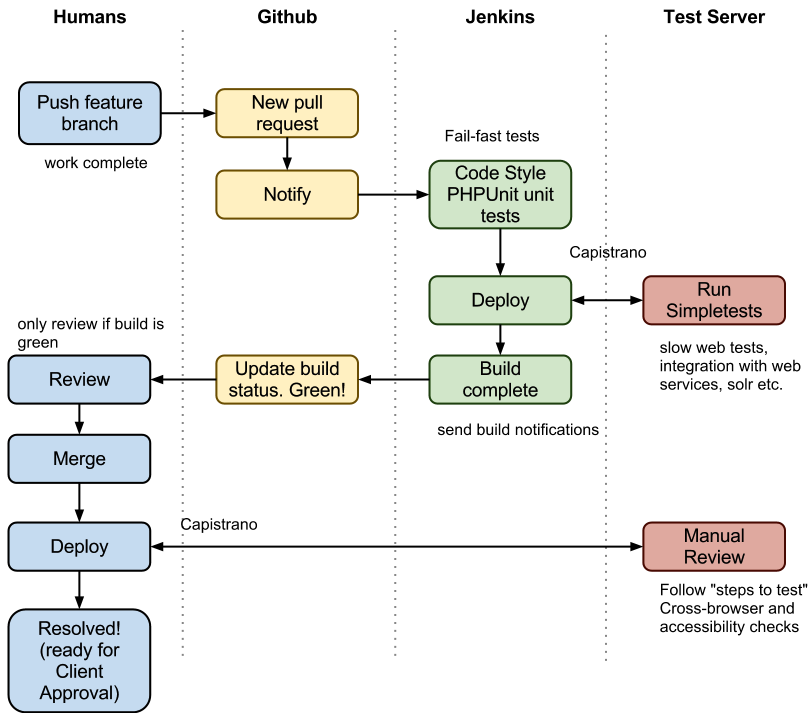
\includegraphics[scale=0.4]{images/osspipeline.png}
	\caption{Pull request delivery pipeline by \cite{osspipeline}}
	\label{fig:osspipeline}
\end{figure}

The only thing to note about the diagram is the manual review as mentioned, this could be automated creating the full continuous delivery pipeline rather than continuous integration.
\\\\
The second system is similar to the pull request however rather than preforming the change in a pull request the commit is placed inside the teams VCS workflow branch. When working in a agile and continuous delivery environment it is general accepted that there should be a master branch that is the latest version of the software. This is also the branch where all the development goes and what the customer gets.
\\\\
Following that system the main branch will have the pipeline attached, when a milestone is reached such as the end of a sprint in agile methodology. A new branch is created to represent the milestone at that point in time. 
\\\\
One reason for this workflow is it will carry well across multiple systems as TFS does not branch in the same way that GIT does. Branching in GIT is similar to changing the entire repository, for example if the current branch is master, then when changing to feature\_one branch it is like renaming the folder and swapping its contents. Think of it like a magic room that changes depending on what branch its on. TFS on the other hand is located on a different path, so rather than a single magic room, its will create a new room for each branch.
\\\\
This difference in design will affect how the automation tool will interact with the VCS, as if it is developed using GIT, the system can watch multiple branches at the same time as it is all located in the same place. Whereas with TFS a new configuration will have to be made for each branch as they are separate from each other.
\\\\
With this in mind, if the workflow used is to create a new branch per version work on it until release then repeat, at the end of every release a new configuration will have to be made for the new branch. While this does not vary from the other workflow in terms of branching, new configuration will not have to be made as they will also be branched off with the project as seen in the next part. But, as development is performed on a single branch there is nothing to change until the project does.
\\\\
Before delving into the why the a new configuration is not needed, the master branch of the project as defied must always be in working condition ready to be delivered the users. If commit are therefore placed directly in master and they make the build or tests fail, then the entire concept of continuous deployment is failed as master is not in a  production ready state.
\\\\
In order to combat this the preferred workflow is to use a feature branches, similar to that of a pull request system, development is performed on another branch then when ready can be merged into the master. Similar this allows tests and other action to be perform on the changes fore they are merged into master. This assures that the master will be kept in a working condition.
\\\\
This will also allow the merge to be reverted if there is an issue in the integration without losing the work performed as more commit can be made and tried to merge again.
\\\\
Now that there is a workflow in place and the pipeline is ready to be attached to the branches, where does the code and other parts needed in the pipeline go. The tools such as Jenkins, Teamcity and cruisecontrol all offer the ability to store scripts inside their systems through their user interface.
\\\\
For example Teamcity comes with pre-scripted runners that will allow a click and select experience to get the entire system set-up. While this is certainly a good selling point for non-experienced or quick one time set-ups over the long term this could be quite the opposite. In multiple ways, if the team decides they want to change from Teamcity to Jenkins now the entire system has to be built from the ground up again. Otherwise it might end up try to fit the way Teamcity handles things into Jenkins.
\\\\
Other issues with software version setting up new branches and so on, there are many more reasons as to why it is good in the short term on small project but for larger and more longer terms a better system is needed.
\\\\
Rather than storing the scripts inside of the tool, they should be placed inside of the VCS then depending on the set up, just have to call a single or multiple external scripts from the tool even if the scripts are a single line. In an ideal situation the scripts should be able to run on the target platforms for the project, such as using python or ruby rather than bash and batch file, to save writing them twice.
\\\\
This also has the befits of someone to walk up to a brand new machine get the repository and have the full system up and running within minutes as the VCS holds all the scripts needed.

\subsection{Hardware architecture}

Up to this point the paper has focused on the software side of thing looking at the pipeline, VCS and scripts. This next section will look at where this is hosted and how where each part can be split.  
\\\\
First thing first the set up will depend on the size of your team and number of build being performed at once, for example a single server will be fine for small teams of five or where as when dealing with hundreds the server also need to scale to match.
\\\\
At the minimum a single server is required, this will hold the VCS, automation tool and staging / testing instance. Finally it will have to include the deployment manager. In general this is a lot of work to place onto a single box and to expect a quick turn feedback timing.
\\\\
Going back to section TODO:CITE on how automation tools work, the general principle is the central server and a lot of registered agents that can take jobs from the sever. This leads nicely into the following architecture seen in figure \ref{fig:bamboo}:

\begin{figure}[H]
	\centering
	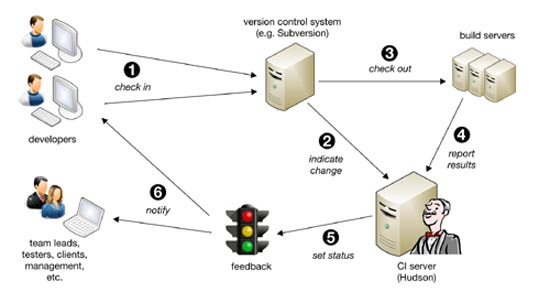
\includegraphics[scale=2.5]{images/bamboo.jpg}
	\caption{Server setup \cite{bamboo}}
	\label{fig:bamboo}
\end{figure}
%https://confluence.atlassian.com/bamboo/understanding-the-bamboo-ci-server-289277285.html

The figure shows that rather than having a single sever it is split into three parts, the first containing the VCS, the second the CI / automation tool, and the third a number of machines to perform the build and tests as necessary.
\\\\
When the build severs are at max capacity new server can be spun up registered to the automation tool then it is good to go. This creates a easily scalable solution that can also be downsized if needed.
\\\\
The main issues with thsi setup is that some of the build server may become specialised. While there may be twenty build servers one may be used for build in linux this creates a bottleneck in the system, ideally all server should be able to accomplish all the task, looking towards Docker or similar programs again for the solution. In order to try and reduce dependency on the machines  and the programs, creating an environment where the system can run on anything quickly.
\\\\
For web application this is general not a problem as the build servers can be set up in way  that is appropriate and reflect the production environment, unless the application is designed to work across different servers such as Linux and windows. This however is not the same for other types of development such as embedded systems.
\\\\
TODO:CITE has designed a work around, interestingly is uses the same principles as Docker, install once and run everywhere, however rather then dealing with software they have recommended to build a software emulator to emulate the target hardware. This emulation can than be ran on any machine allowing the once specialise system to be generalised over multiple servers, removing the bottleneck. This designed can be seen in figure \ref{fig:intel}:

\begin{figure}[H]
	\centering
	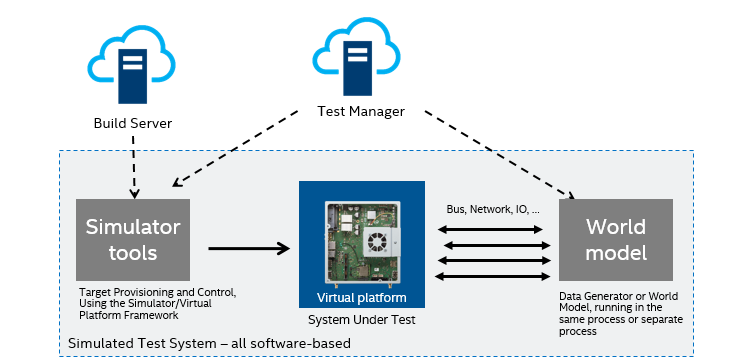
\includegraphics[scale=0.7]{images/intel.png}
	\caption{Embedded systems \cite{intel}}
	\label{fig:intel}
\end{figure}
% https://software.intel.com/en-us/blogs/2017/03/13/continuous-delivery-embedded-systems-and-simulation

In this part most of the solution are focused on self-hosted and run solutions, however there is also the option to rent or buy the whle package rather then run them internally. For example, GihHub, BitBucket and GitLab provide a was to host GIT repositories, at a price, they even offer intergeneration with CI services such as Travis. 
\\\\
Cloudbees, BitbucketPipelines and others offers a cloud solution to take the repository and perform the operation on then removing the need to worry about servers and interaction between them. Untimely the choice of system will come down to the project and budget at hand. With sensitive data, a self-hosted solution will work out better whereas a open source project will fair well with the cloud solutions.
\\\\
While the cloud solutions remove the need for handling the severs and sever set up themselves, the architecture discussed in the section will still apply as there will still be a need for a VCS server and automation tool server, it is just a matter of not dealing with them directly, but rather though a third party.

\subsection{Deployment}
\label{sec:deployment}

Up till this point the paper has covered all the parts within the pipeline apart from deployment, and how to deploy a system from the end of the pipeline. This next part aims to cover this.

\subsubsection{Databases}
Sometimes no matter what application it is will have some form of database in the background, when the application updates, so the the database, changing the schema, tables and so on. In a continuous delivery pipeline this could happen multiple times in a day, whist trying to hold to the zero downtime expectations
\\\\
TODO:CITE has designed a application that achieves just that on a small scale, the paper also lists several alternatives that try and accomplish this. This is an on going area of research and should be expanded on to get the process to be as smooth as possible without disrupting the running of the application.  

\subsubsection{Servers}

Servers are unique as in general the company creating the product will also host or manage the server, this creates an easy situation where the entire pipeline is an internal process with minimal external needs, such as with the server company like Amazon web services (AWS).
\\\\
With a standard set-up the new version should be deployed behind the scenes then once done so the live site should now direct the the newer version rather tan the old. This can create an easy fall-back system if something goes completely wrong.
\\\\
The can be done by setting up another Docker container, or however the application is designed to be deployed, it is key however to have this automated. With regards to the database, idealy the database should be handled separately from the rest of the application to minimise errors. And when falling back to not have data loss.
\\\\
The deployment of servers are the type to be handled by the likes of Octopus, chef and puppet. That is not to say that they cannot be used for other type of deployment, more so that is where they are specialised.

\subsubsection{Downloadable applications}

As far as downloadable application or desktop applications, there are multiple options open, the main idea is to provide a area that can be check and downloaded via the software, by bundling the software up. On Linux type operating system (OS) this is normally checking the bundled software in to the package control repository, and updated via the system package manager such as apt-get or Pacman. 
\\\\
However, on a Windows like OS, even possible on Linux there are multiple option open to handle the updating of software TODO:CITE covers this, the final choice will come down to the type of software that is being deployed, a web browser can update and install in the background with the users knowledge fine, however more critical software must not, and must be handled with great care.

\subsubsection{Mobile applications}

Similarly, to Linux like application there is normally a gatekeeper in the way of pushing update directly to the user and instead must go through the "store". Therefore the deployment stage will consist of packaging the software up and submitting it to the store. 
\\\\
The ability to automate this process is not so much down to the software but rather the gatekeeper, as they may have manual review and delayed times between submissions, while internally continuous deployment can be used the gate keeper may make it impossible to do so all the way to the user.

\subsection{Architecture final thoughts}

Overall, there are some very clear structures and patterns to be found when creating a continuous deployment system. Starting with the pipeline, emerging two main styles of transporting depending on the type of application.
\\\\
To the workflow around the pipeline ensuring that there is a master breach that is always in development and the practises around them. Either through the uses of a pull request or feature branch system.
\\\\
Then onwards to the hardware and server set with the ideal three tier set up, allowing easy expansion and reduction of servers as needed. Ensuring that each of the servers a generalised as to be any to run any task. Even those on specialised hardware. Including the opportunity to use other hosted services.
\\\\
Following on to the best practises around the deployment of the system for three different types of applications, web, downloadable and mobile.  
\\\\
While the final project may vary from depending on what part are used, the core principles, design and work flow found here should be used as the backbone of creating a continuous delivery or continuous integration system.
	%
% The MIT License (MIT)
%
% Copyright (c) 2017 Paul Batty
%
% Permission is hereby granted, free of charge, to any person obtaining a copy
% of this software and associated documentation files (the "Software"), to deal
% in the Software without restriction, including without limitation the rights
% to use, copy, modify, merge, publish, distribute, sublicense, and/or sell
% copies of the Software, and to permit persons to whom the Software is
% furnished to do so, subject to the following conditions:
%
% The above copyright notice and this permission notice shall be included in
% all copies or substantial portions of the Software.
%
% THE SOFTWARE IS PROVIDED "AS IS", WITHOUT WARRANTY OF ANY KIND, EXPRESS OR
% IMPLIED, INCLUDING BUT NOT LIMITED TO THE WARRANTIES OF MERCHANTABILITY,
% FITNESS FOR A PARTICULAR PURPOSE AND NONINFRINGEMENT. IN NO EVENT SHALL THE
% AUTHORS OR COPYRIGHT HOLDERS BE LIABLE FOR ANY CLAIM, DAMAGES OR OTHER
% LIABILITY, WHETHER IN AN ACTION OF CONTRACT, TORT OR OTHERWISE, ARISING FROM,
% OUT OF OR IN CONNECTION WITH THE SOFTWARE OR THE USE OR OTHER DEALINGS IN
% THE SOFTWARE.
%

\section{Evaluation}
\label{sec:evaluation}

eval
	%
% The MIT License (MIT)
%
% Copyright (c) 2017 Paul Batty
%
% Permission is hereby granted, free of charge, to any person obtaining a copy
% of this software and associated documentation files (the "Software"), to deal
% in the Software without restriction, including without limitation the rights
% to use, copy, modify, merge, publish, distribute, sublicense, and/or sell
% copies of the Software, and to permit persons to whom the Software is
% furnished to do so, subject to the following conditions:
%
% The above copyright notice and this permission notice shall be included in
% all copies or substantial portions of the Software.
%
% THE SOFTWARE IS PROVIDED "AS IS", WITHOUT WARRANTY OF ANY KIND, EXPRESS OR
% IMPLIED, INCLUDING BUT NOT LIMITED TO THE WARRANTIES OF MERCHANTABILITY,
% FITNESS FOR A PARTICULAR PURPOSE AND NONINFRINGEMENT. IN NO EVENT SHALL THE
% AUTHORS OR COPYRIGHT HOLDERS BE LIABLE FOR ANY CLAIM, DAMAGES OR OTHER
% LIABILITY, WHETHER IN AN ACTION OF CONTRACT, TORT OR OTHERWISE, ARISING FROM,
% OUT OF OR IN CONNECTION WITH THE SOFTWARE OR THE USE OR OTHER DEALINGS IN
% THE SOFTWARE.
%

\section{Conclusion}
\label{sec:conclusion}

At the start of the paper, several goals where defined. The first to look at and understand the terminology, history and meaning behind the various forms of continuous integration, continuous deployment and automatic build and the surround culture of devops. This was achieved in the first chapter of this paper.
\\\\
The second was to look at examples and other implementations of such system in the real world, taking a look at what went right, what they have in common and deriving the ideal systems from theses studies. This was achieved in the second and third chapters.
\\\\
Thirdly, to look at the cost benefits and who should use such as system in the first place, while looking at the status of the current situation around devops and where it is heading, making sure that it is on track. This took on the role looking at what is missing from the toolset and where thing have been done right.
\\\\
Overall, this project has been a success. The aims set out at the start have been achieved. There are a few minor issues that could be improved upon such as using more case studies to create a better foundation on which to draw from. 
\\\\
In the future, more time should be spend towards looking at creating easily reproducible and testing environments for embedded systems as they are non-existant when compared to the status of web, desktop and mobile development.
\\\\
But, this has been an enjoyable and successfully project and having learnt a great deal about the various technology stacks such as Docker, Vagrant and some of the more unique style of application such as serverless servers. In addition to a guide of which can be used when needed to implement a variation of  such a system
	%
% The MIT License (MIT)
%
% Copyright (c) 2017 Paul Batty
%
% Permission is hereby granted, free of charge, to any person obtaining a copy
% of this software and associated documentation files (the "Software"), to deal
% in the Software without restriction, including without limitation the rights
% to use, copy, modify, merge, publish, distribute, sublicense, and/or sell
% copies of the Software, and to permit persons to whom the Software is
% furnished to do so, subject to the following conditions:
%
% The above copyright notice and this permission notice shall be included in
% all copies or substantial portions of the Software.
%
% THE SOFTWARE IS PROVIDED "AS IS", WITHOUT WARRANTY OF ANY KIND, EXPRESS OR
% IMPLIED, INCLUDING BUT NOT LIMITED TO THE WARRANTIES OF MERCHANTABILITY,
% FITNESS FOR A PARTICULAR PURPOSE AND NONINFRINGEMENT. IN NO EVENT SHALL THE
% AUTHORS OR COPYRIGHT HOLDERS BE LIABLE FOR ANY CLAIM, DAMAGES OR OTHER
% LIABILITY, WHETHER IN AN ACTION OF CONTRACT, TORT OR OTHERWISE, ARISING FROM,
% OUT OF OR IN CONNECTION WITH THE SOFTWARE OR THE USE OR OTHER DEALINGS IN
% THE SOFTWARE.
%

\section*{References}
\label{sec:references}

\begin{thebibliography}{0}

% order aphabeticaly by first name.
\bibitem[Jong M. Deursen† A., 2015]{updatedatabse}
Jong M., Deursen† A. (2015), Continuous Deployment and Schema Evolution in SQL Databases, Delft University of Technology, Delft, The Netherlands
\\
\bibitem[Atlassian, 2017]{bamboo}
Atlassian. (2017), On line publication, Understanding the Bamboo CI Server, https://confluence.atlassian.com/bamboo/understanding-the-bamboo-ci-server\\-289277285.html, Last Accessed 23rd May 2017
\\
\bibitem[Berczuk S. Appleton B., 2002]{unit_tests}
Berczuk S., Appleton B. (2002), Software Configuration Management Patterns: Effective Teamwork, Practical Integration, Boston, ISBN 0201741172.
\\
\bibitem[Vassallo C. Zampetti F. Romano D., 2016]{CIF}
Vassallo C., Zampetti F., Romano D. (2016), Continuous Delivery Practices in a Large Financial Organization,In Proceedings of 2016 IEEE International Conference on Software Maintenance and Evolution, Raleigh, NC, USA, October 2 - 7, 2016, 519-528.
\\
\bibitem[Smith D., 2014]{XPH}
Smith D. (2014), On line publication, Extreme Programming (XP), http://projectmanagementhistory.com/Extreme\_Programming\_(XP).html, Last Accessed 22th May 2017
\\
\bibitem[Wells D., 1999]{XP}
Wells D. (1999), On line publication, Extreme programming: A gentle introduction, http://www.extremeprogramming.org/, Last Accessed 20th April 2017
\\
\bibitem[Engblom J., 2017]{intel}
Engblom J. (2017), On line publication, Continuous Delivery, Embedded Systems, and Simulation, https://software.intel.com/en-us/blogs/2017/03/13/continuous-delivery-embedde\\d-systems-and-simulation, Last Accessed 23rd May 2017
\\
\bibitem[Fournova Software, 2013]{VCSSYSTEMS}
Fournova Software. (2013), On line publication, Switching from Subversion to Git, https://www.git-tower.com/learn/git/ebook/en/command-line/appendix/\\from-subversion-to-git, Last Accessed 25th April 2017
\\
\bibitem[Fitz T., 2009]{deploy}
Fitz T. (2009), On line publication, Continuous Deployment for Downloadable Client Software, http://timothyfitz.com/2009/03/09/cd-for-client-software/, Last Accessed 23rd May 2017
\\
\bibitem[Hanna T., 2016]{cc}
Hanna T. (2016), On line publication, Comparing CI servers: Jenkins vs. CruiseControl vs. Travis, https://jaxenter.com/comparing-vi-servers-jenkins-vs-cruise-control-vs-travis-12\\5426.html, Last Accessed 22th May 2017
\\
\bibitem[Pepper K., 2013]{osspipeline}
Pepper K. (2013), On line publication, Automated Drupal Testing with Github Pull Requests, https://www.previousnext.com.au/blog/automated-drupal-testing-github-pull-re\\quests, Last Accessed 9th May 2017
\\
\bibitem[Fowler M., 2006]{mf}
Fowler M. (2006),  On line publication, Continuous Integration, https://martinfowler.com/articles/continuousIntegration.html, Last Accessed 22th May 2017
\\
\bibitem[Rapaport R., 2014]{devop_history}
Rapaport R. (2014), On line publication, A Short History of DevOps, https://www.ca.com/us/rewrite/articles/devops/a-short-history-of-devops.html, Last Accessed 22th May 2017
\\
\bibitem[Stackoverflow, 2017]{vcspop}
Stackoverflow. (2017), On line publication, Developer survey results, http://stackoverflow.com/insights/survey/2017\#work-version-control, Last Accessed 25th April 2017
\\
\bibitem[Karadzhov S., 2014]{zend}
Karadzhov S. (2014), On line publication, Fundamentals of Continuous Integration with Jenkins and zend server, http://static.zend.com/topics/WP-Fundamentals-of-Continuous-Integration-with\\
-Jenkins-and-Zend-Server-2014-03-31-EN.pdf, Last Accessed 4st May 2017
\\
\bibitem[Vaughan-Nichols S., 2014]{docker-vm}
Vaughan-Nichols S. (2014), On line publication, What is Docker and why is it so darn popular?, http://www.zdnet.com/article/what-is-docker-and-why-is-it-so-darn-popular/, Last Accessed 1st May 2017
\\
\bibitem[Mansoor U., 2016]{codeahoy}
Mansoor U. (2016), On line publication, Continuous Delivery - Automating the Release Process, https://codeahoy.com/2016/06/18/continuous-delivery-automating-the-release-\\process/, Last Accessed 5th May 2017
\\
\bibitem[Naik V., 2016]{thoughworks}
Naik V., (2016), On line publication, Architecting for Continuous Delivery, https://www.thoughtworks.com/insights/blog/architecting-continuous-delivery, Last Accessed 5th May 2017

\end{thebibliography}
	%
% The MIT License (MIT)
%
% Copyright (c) 2017 Paul Batty
%
% Permission is hereby granted, free of charge, to any person obtaining a copy
% of this software and associated documentation files (the "Software"), to deal
% in the Software without restriction, including without limitation the rights
% to use, copy, modify, merge, publish, distribute, sublicense, and/or sell
% copies of the Software, and to permit persons to whom the Software is
% furnished to do so, subject to the following conditions:
%
% The above copyright notice and this permission notice shall be included in
% all copies or substantial portions of the Software.
%
% THE SOFTWARE IS PROVIDED "AS IS", WITHOUT WARRANTY OF ANY KIND, EXPRESS OR
% IMPLIED, INCLUDING BUT NOT LIMITED TO THE WARRANTIES OF MERCHANTABILITY,
% FITNESS FOR A PARTICULAR PURPOSE AND NONINFRINGEMENT. IN NO EVENT SHALL THE
% AUTHORS OR COPYRIGHT HOLDERS BE LIABLE FOR ANY CLAIM, DAMAGES OR OTHER
% LIABILITY, WHETHER IN AN ACTION OF CONTRACT, TORT OR OTHERWISE, ARISING FROM,
% OUT OF OR IN CONNECTION WITH THE SOFTWARE OR THE USE OR OTHER DEALINGS IN
% THE SOFTWARE.
%

\section{Appendix}
\label{sec:appendix}
\end{document}